\documentclass[letterpaper,10pt,draftclsnofoot,onecolumn,]{article}
\usepackage[utf8]{inputenc}
\usepackage[margin=0.75in]{geometry}
\usepackage{tikz}
\usepackage{array}
\usepackage{graphicx}
\usepackage{booktabs}
\usepackage{float}
\begin{document}
\noindent
\begin{titlepage}
    \begin{center}
        \vspace*{1cm}
        
        \textbf{\huge{Gymnastics Scoring Software}}
        
        \vspace{0.5cm}
        \large{The purpose of this paper is to define the design for the proposed gymnastics scoring software.}
        
        \vspace{1.5cm}
        
        \textbf{\LARGE{10.0 Software}}
        
        \Large{Design Document\\
        CS 461\\
        Senior Software Engineering Project\\
        Fall 2018}
        \vspace*{\fill}
        \begin{center}
            \textbf{\large{Abstract}}
        \end{center}
        \normalsize{This document archives the in depth technical and design choices made by 10.0 Software for our competitive gymnastics scoring software. Continuing, this document shows systems through the use of UMLs to visually show the classes, objects, systems, and how all of the systems are interconnected. Moreover, this document touches on the topics of conceptual models, design descriptions, and design viewpoints to further show and document how the system works.}
    \end{center}
\end{titlepage}

\tableofcontents
\newpage

%Change Log
\begin{table}[htbp]
    \centering
    \small
    \setlength\tabcolsep{2pt}
    \caption{Change Log}
    \label{tab:change-log}
    \begin{tabular}{p{4em} p{25em} p{25em}}
        \toprule
        Section & Original                                              & New                                \\ \midrule
        4.6     & Required input of JSON Files.                         & Can use JSON files or Manual input. \\
        4.8     & Mentioned Microsoft SQL.                              & Changed Microsoft SQL to just SQL. \\
        5.4.1   & Teams endpoint object and description                 & Teams moved to 5.4.6 and 5.4.1 is now judge endpoint object and description. \\
        5.4.2   & Players endpoint object and description               & Players moved to 5.4.4 and 5.4.2 is now lineup endpoint object and description. \\
        5.4.3   & Events endpoint object and description                & Events endpoint was removed and replaced with meet endpoint object and description. \\
        5.4.4   & Nothing.                                              & Player endpoint object and description. \\
        5.4.5   & Nothing.                                              & Score endpoint object and description. \\
        5.4.6   & Nothing.                                              & Team endpoint object and description. \\
        5.4.7   & Nothing.                                              & User endpoint object and description. \\
        5.6     & UML diagram of database.                              & Reworked database and changed UML diagram to an Entity Relationship Diagram that more accurately shows the database. \\
        5.8     & No screenshots.                                       & Added Screenshots .                 \\
        5.11    & Originally required a printing feature and XML export.& Removed printing and XML exporting. \\
        5.12    & Originally didn't have average score algorithm.       & Added average score algorithm.      \\
        5.13    & Nothing here .                                        & Added NPM modules and descriptions. \\
        \bottomrule
    \end{tabular}
\end{table}

% Section 1
\section{Overview}
\subsection{Scope}
This document details the plans to implement the Gymnastics Scoring Software. To accomplish these goals a system will be implemented that consists of a database, web portal, API, printer interface, and an interface with the scoreboard inside Gill Colosseum. 
\subsection{Purpose}
The purpose of this system is to provide an improved viewing experience for OSU Gymnastics spectators as well as making the scoring process easier for the judges and data inputters.This document will provide detailed information on the implementation of the Gymnastics Scoring Software. The document will detail the implementation of the database, web portal, API, and scoreboard interface. 
\subsection{Intended audience}
This document is intended for the IT team at Gill Colosseum and anyone responsible for the implementation of this system. 

\subsection{Conformance}
Firstly, we shall make set-up time for a meet to be under a half hour. Secondly, we shall make sure that the scoring and results are correct to NCAA gymnastics standards. Thirdly, we shall make sure that the program is able to update the scoreboards and display peripherals in a timely manner. Fourthly, we shall ensure that our program can successfully print out the meet score sheet at any point during the gymnastics meet. Fifthly, we shall make sure that our program can export the data from the meet to the Road to Nationals database as required by the NCAA.
% Section 1

% Section 2
\section{Definitions}
\begin{center}
    \begin{tabular} { | p{10em} | p{40em} | }
    \hline
    \textbf{Term} & \textbf{Definition} \\
    \hline
    V/B/B/F & Vault, Bar, Beams, and Floor. The four events in gymnastics are commonly grouped together. When V/B/B/F is used it means that each will have an individual variable. \\
    \hline
    SDD & Software Design Description. \\
    \hline
    Admin (authentication level) & The highest level of authentication. Moderators have the ability to set-up teams, meets, and delete data. \\
    \hline
    Scorer (authentication level) & The lowest level of authentication, Judge stands for the accounts that will be in charge of inputting singular judges scores. Judge level accounts are able to input scores and get gymnast and team data. \\
    \hline
    UML & Unified Modeling Language. \\
    \hline
    API & Application Programming Interface. \\
    \hline
    \end{tabular}
\end{center}

% Section 2

% Section 3
\section{Conceptual model for software design descriptions}
% This clause establishes a conceptual model for SDDs. The conceptual model includes basic terms and concepts of SDD, the context in which SDDs are prepared and used, the stakeholders who use them, and how they are used. 

\subsection{Software design in context}
For the gymnastics scoring software project, an object oriented design method will be used. Self-contained entities such as gymnast, team, and event will be contained in objects. Design relationships such as encapsulation, specialization, and composition will be used to implement the scoring application. We will construct a design viewpoint to show design elements. A design elements consists of four categories: design constraints, design relationships, design attributes, and design entities. The design viewpoints will specify the design elements and conventions for the design views that it governs. Each design view contains multiple entities, attributes for the entities, relationships between entities, and constraints on those design elements. Stakeholders of the gymnastics scoring software project can obtain the information they need through these design views.
% View in reference it is about 4 pages long
\subsection{Software design descriptions within the life cycle}
\subsubsection{Influences on SDD preparation}
The most important factor to the SDD is the requirements document.The design decisions and design constraints are based on the contents of the requirements document.
\subsubsection{Influences on software life cycle products}
The SDD can influence change in the requirements document and test documentation. During the process of creating the SDD, we may discover through design decisions or design constraints that the requirement document needs changes. When we create test cases and test procedures, we will need to consider the SDD.
\subsubsection{Design verification and design role in validation}
The SSD will be tested through design verification to find out if the design properly meets the stakeholders' design requirements and covers demanded design choices. Design concerns may be discovered through verification. The verification process can done through analysis, inspection, or review. The design role in validation is presenting an overview of how the system will work, the reasoning behind the design choices, and  how the design traces to the requirements document. 
% In this standard, a typical cycle will be used to describe the various design situations in which an SDD can be created and used. This life cycle is based on IEEE Std 12207-2008 [B21]. 
% Section 3

% Section 4
\section{Design description information content}
\subsection{Introduction}
The design description information content section will describe the identification of the software design description, identified design stakeholders, identified design concerns, selected design viewpoints, design views, design overlays, and design rationale. Each of the design viewpoints will have type definitions of its allowed design elements and design languages.
languages  
\subsection{SDD identification}\\

\quad{- Date of issue and status}\\
The design document date of issue is November 27, 2018. The current status of the design document is 2nd draft.\\

- Scope\\
The scope of the 10.0 Software design description is the design of the web portal, API, and database, and how each of those components interact.\\

- Issuing organization\\
This project was issued by Oregon State Gymnastics which is a part of Oregon State Athletics.\\

- Authorship\\
The members of group 18 will create and own the gymnastics scoring software (10.0 Software). There are currently no plans for any copyrights.\\

- Context\\
We are designing 10.0 Software to replace the scoring software that is currently being used for gymnastics meets in Gill Coliseum because it is outdated and has problems such as a long set up time and reliability issues.\\

- Design languages for design viewpoints\\
We will use UML for context, composition, logical, dependency, information, patterns, interface, structure, interaction, state dynamics, algorithm, and resources.\\

- Body\\
The software design description for this system includes the web portal, API, database, and scoreboard server components and how they interact with each other. For the design of this gymnastics scoring software (10.0 Software), how the components interact will require most of the description. The purpose of each component is to interact with and possibly provide an interface for other components. The API is an interface for the web portal to access the database and the scoreboard server. The web portal will provide and interface for the users to use the whole system.\\

- Change history\\
The 10.0 Software project does not have a change history yet since it is still in the design phase.

\subsection{Design stakeholders and their concerns}
\quad{- Stakeholders}\\
The stakeholder for 10.0 Software is the associate head coach of the Oregon State gymnastics team, Michael Chaplin and Gill Coliseum IT.\\

- Stakeholder concerns\\
The design concerns of the stakeholders are that SQL should be used for the database, that the software is designed in a way that the setup time before meets takes no longer than 30 minutes, and that it is designed so that the user can easily run the web portal.\\

- Addressed concerns\\
The system is designed with a SQL database. The setup is designed so that the user can upload a JSON file with the gymnasts on a team instead of having to input each gymnast on each team which will save time for the setup. The web portal is designed in such a way that the user can easily run it by making it as simple as possible while still providing the necessary functionality.

\subsection{Design views}
This project has three design views based on the concerns of the stakeholders. The three design views are focusing on setup time, web portal usability, and a SQL database.

\subsection{Design viewpoints}
\quad{- Viewpoint name}\\
The name of the first viewpoint is setup.\\

- Design concerns\\
The setup time of the software for a gymnastics meet must take thirty minutes or less.\\

- Design elements\\
The user will use the web portal to set up the meet. Specifically, the meet setup page and the team setup page of the web portal will be used. The setup design viewpoint does not allow for the user to input one gymnast at a time because that may take longer than thirty minutes. Instead, the user will give a JSON file for each team with the gymnasts on that team for team setup.\\

- Analytical method\\
The method used to construct the setup time design view is to make design choices based on how much time they add to the setup.\\

- Viewpoint name\\
The name of the second viewpoint is usability.\\

- Design concerns\\
The web portal must be efficient and easy for the user to run 10.0 Software with.\\

- Design elements\\
The web portal is the main element for usability because that is the only part the user interacts with.\\

- Analytical method\\
The method used to construct the usability design view is to make design choices with the user in mind.\\

- Viewpoint name\\
The name of the third viewpoint is database.\\

- Design concerns\\
The software must use a SQL database.\\

- Design elements\\
The database is the main design element for the database viewpoint but the API is a secondary element since it interacts with the database.\\

- Analytical method\\
The method used to construct the database design view is to make design choices using a relational database.

\subsection{Design elements}
\begin{itemize}
    \item \textbf{Web Portal}: The web portal is where the user interacts with the system for entering scores, printing, and displaying information on the scoreboard.
    \item \textbf{Setup}: The setup element requires the user to insert data about both meets and teams.
    \item \textbf{API}: The API is the logical process responsible for reacting to user requests.
    \item \textbf{Database}: The SQL database hosted on Gill Coliseum's server will store all team and gymnast related data.
\end{itemize}
\subsection{Design overlays}
Security and authentication are also important to the stakeholders and are therefore an area of focus in the design of 10.0 Software.
\subsection{Design rationale}
We decided to use a Microsoft SQL database and web portal for our gymnastics scoring software. An important stakeholder concern is ease of use. We think that implementing a web application with a SQL database as the backbone will make the system very user friendly as well as fast to set up especially compared to the current system. A desktop application to score the gymnasts was also considered, but we felt the web application fits our purpose better. A design concern is that the stakeholders may want to make changes to the system after testing it and the web application would be simpler to change. In the more distant future, the web application can be continually upgraded with new features easily. We decided to use a SQL based database because that is what the Gill IT staff wanted. The fast set up time design concern was addressed by allowing users to input a JSON file with the team rosters.
\subsection{Design languages}
The selected design language for our software design description is UML. The three primary categories of UML diagrams are structure diagrams, behavior diagrams, and interaction diagrams. We will use UML to clarify design viewpoints. 
% Section 4

% Section 5
\section{Design viewpoints}
\subsection{Introduction}
\begin{center}
\textbf{Table 1---Summary of design viewpoints}
\begin{tabular}{| p{10em} | p{20em} | p{20em} |}
\hline
\textbf{Design Viewpoint} & \textbf{Design concerns} & \textbf{Example design languages} \\
\hline
Context (5.2) & Gill coliseum IT people, judge assistants/OSU gymnastic data inputters & UML use case diagrams \\
\hline
Composition (5.3) & SQL database, API server, client side web portal, scoreboard server & UML package diagram and UML component diagram \\
\hline
Logical (5.4) & endpoints will act as classes due as they will call functions and use data & UML class diagram and UML object diagram \\
\hline
Dependency (5.5) & npm modules, endpoints, and web server & UML package diagrams and component diagrams \\
\hline
Information (5.6) & Persistent data will need to be constantly reordered and updated as a meet is under progress & UML class diagram\\
\hline
Patterns (5.7) & Multiple endpoints that allow for abstraction of data to make simple and effective API calls & UML composite structure diagram\\
\hline
Interface (5.8) & Web portal & UML component diagram\\
\hline
Structure (5.9) & HTTP server structure with a client-server architecture & UML structure and class diagram\\
\hline
Interaction (5.10) & The client will interact with the server, the server will interact with the scoreboard server, printing service, and client & UML sequence and communication diagram\\
\hline
State dynamics (5.11) & Setting up meets based on number of teams and judges present & UML state machine diagram\\
\hline
Algorithm (5.12) & It needs to be quick enough to display scores before fans get restless & Decision tale\\
\hline
Resources (5.13) & npm modules & UML\\
\hline
\end{tabular}
\end{center}
\subsection{Context viewpoint}
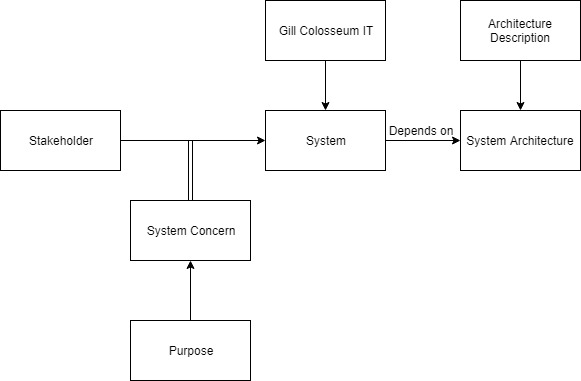
\includegraphics[width=\textwidth,height=\textheight,keepaspectratio]{contextdiagram}
\subsection{Composition viewpoint}
This system is made up of 5 components which are the web portal, API, database, printer interface and scoreboard interface. The API is the core of the system and is responsible for communication between the user at the web portal with the printer, scoreboard, and database. The web portal allows the user to access the database as well as printing and scoreboard features.\\
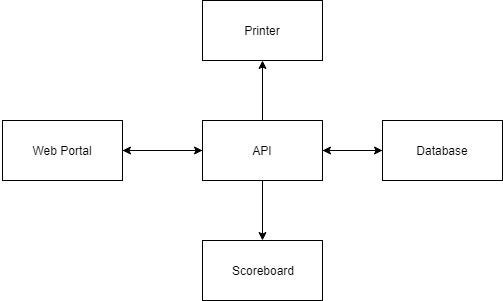
\includegraphics[width=\textwidth,height=\textheight,keepaspectratio]{compositiondiagram}
\subsection{Logical viewpoint}
Due to the use of a HTTP server and client-server architecture classes are not primarily present, and are instead replaced with server endpoints. Three major endpoints will be used: teams, events, and gymnasts.
\subsubsection{/judge}
\begin{center}
    \begin{tabular}{| p{20em} |}
        \hline
        \textbf{/judge} \\
        \hline
        - int: id \\
        - varchar: name \\
        - int: meetID \\
        \hline
        + GET /judge \\
        + GET /judge/meet/:meetID \\
        + POST /judge \\
        + PUT /judge/:judgeID \\
        + DELETE /judge/:judgeID \\
        \hline
    \end{tabular}
\end{center}
\begin{center}
    \begin{tabular}{ | p{15em} | p{8em} | p{7em} | p{20em} | }
    \hline
    \textbf{Name} & \textbf{Return} & \textbf{Authentication level} & \textbf{Definition} \\
    \hline
    GET /judge & judge[] & None & Returns a list of all judges in the database. \\
    \hline
    GET /judge/meet/:meetID & Judge[] & None & Returns a list of all judges that participated in the meet specified by :meetID. \\
    \hline
    POST /judge & Status code 201 & Admin & Creates a judge object in the database. Data is grabbed from the body of the request sent to the server. \\
    \hline
    PUT /judge/:judgeID & Status code 204 & Admin & Updates the judge object specified by :judgeID. \\
    \hline
    DELETE /judge/:judgeID & Status code 204 & Admin & Deletes the judge object specified by :judgeID. \\
    \hline
    \end{tabular}
\end{center}
\subsubsection{/lineup}
\begin{center}
    \begin{tabular}{| p{22em} |}
        \hline
        \textbf{/lineup} \\
        \hline
        - int: id \\
        - int: playerID \\
        - int: teamID \\
        - int: order \\
        - varchar: event \\
        - int: meetID \\
        \hline
        + GET /lineup/:meetID/:teamID/:event \\
        + GET /lineup/score/:meetID/:teamID/:event \\
        + POST /lineup \\
        + PUT /lineup/:lineupID \\
        + DELETE /lineup/:lineupID \\
        \hline
    \end{tabular}
\end{center}
\begin{center}
    \begin{tabular}{ | p{15em} | p{8em} | p{7em} | p{20em} | }
        \hline
        \textbf{Name} & \textbf{Return} & \textbf{Authentication level} & \textbf{Definition} \\
        \hline
        GET /lineup/:meetID/:teamID/:event & Lineup[] & None & Returns the lineup for the meet specified by :meetID, the team specified by :teamID, and the event specified by :event. \\
        \hline
        GET /lineup/score/:meetID/:teamID /:event & Float & None & Returns the score of the top five gymnasts for the lineup for the meet specified by :meetID and the team specified by :teamID. \\
        \hline
        POST /lineup & Status code 204 & Admin & Creates a new lineup object. \\
        \hline
        PUT /lineup/:lineupID & Status code 204 & Admin & Updates the lineup object specified by :lineupID. \\
        \hline
        DELETE /lineup/:lineupID & Status code 204 & Admin & Deletes the lineup object specified by :lineupID. \\
        \hline
    \end{tabular}
\end{center}
\subsubsection{/meet}
\begin{center}
    \begin{tabular}{| p{20em} |}
        \hline
        \textbf{/meet} \\
        \hline
        - int: id \\
        - varchar: name \\
        \hline
        + GET /meet \\
        + GET /meet/:meetID \\
        + POST /meet \\
        + PUT /meet/:meetID \\
        + DELETE /meet/:meetID \\
        \hline
    \end{tabular}
\end{center}
\begin{center}
    \begin{tabular}{ | p{15em} | p{8em} | p{7em} | p{20em} | }
        \hline
        \textbf{Name} & \textbf{Return} & \textbf{Authentication level} & \textbf{Definition} \\
        \hline
        GET /meet & Meet[] & None & Returns an array of all meets in the database. \\
        \hline
        GET /meet/:meetID & Meet & None & Returns a single meet object specified by :meetID. \\
        \hline
        POST /meet & Status code 204 & Admin & Creates a new meet object. \\
        \hline
        PUT /meet/:meetID & Status code 204 & Admin & Updates the meet object specified by :meetID. \\
        \hline
        DELETE /meet/:meetID & Status code 204 & Admin & Deletes the meet object specified by :meetID. \\
        \hline
    \end{tabular}
\end{center}
\subsubsection{/player}
\begin{center}
    \begin{tabular}{| p{20em} |}
        \hline
        \textbf{/player} \\
        \hline
        - int: id \\
        - int: playerNum \\
        - varchar: name \\
        - int: teamID \\
        - float: vaultScore \\
        - float: barScore \\
        - float: beamScore \\
        - float: floorScore \\
        - float: AAScore \\
        - int: meetID \\
        \hline
        + GET /player/:meetID/:teamID \\
        + GET /player/:playerID \\
        + GET /player/:playerID/:event \\
        + POST /player \\
        + PUT /player/:playerName \\
        + DELETE /player/:playerID \\
        \hline
    \end{tabular}
\end{center}
\begin{center}
    \begin{tabular}{ | p{15em} | p{8em} | p{7em} | p{20em} | }
        \hline
        \textbf{Name} & \textbf{Return} & \textbf{Authentication level} & \textbf{Definition} \\
        \hline
        GET /player/:meetID/:teamID & Player[] & None & Gets the players for the meet specified by :meetID and the team specified by :teamID. \\
        \hline
        GET /player/:playerID & Player & None & Gets the player object specified by :playerID. \\
        \hline
        GET /player/:playerID/:event & Float & None & Gets the score of the player object specified by :playerID for the event specified by :event. \\
        \hline
        POST /player & Status code 204 & Admin & Creates a player object. \\
        \hline
        PUT /player/:playerID & Status code 204 & Admin & Updates the player object specified by :playerID. \\
        \hline
        DELETE /player/:playerID & Status code 204 & Admin & Deletes the player object specified by :playerID. \\
        \hline
    \end{tabular}
\end{center}
\subsubsection{/score}
\begin{center}
    \begin{tabular}{| p{22em} |}
        \hline
        \textbf{/score} \\
        \hline
        - int: id \\
        - int: playerID \\
        - int: judgeID \\
        - float: score \\
        - varchar: event \\
        - boolean: exhibition \\
        - int: meetID \\
        \hline
        + GET /score \\
        + GET /score/meet/:meetID \\
        + GET /score/average/:meetID/:playerID/:event \\
        + POST /score \\
        + PUT /score/:scoreID \\
        + DELETE /score/:scoreID \\
        \hline
    \end{tabular}
\end{center}
\begin{center}
    \begin{tabular}{ | p{15em} | p{8em} | p{7em} | p{20em} | }
        \hline
        \textbf{Name} & \textbf{Return} & \textbf{Authentication level} & \textbf{Definition} \\
        \hline
        GET /score & Score[] & None & Returns all of the scores in the database. \\
        \hline
        GET /score/meet/:meetID & Score[] & None & Returns all of the scores for the meet specified by :meetID. \\
        \hline
        GET /score/average/:meetID/:playerID /:event & Float & None & Returns the average score for the player specified by :playerID from the meet specified by :meetID for the event specified by :event. \\
        \hline
        POST /score & Status code 204 & Admin or Scorer & Creates a score object \\
        \hline
        PUT /score/:scoreID & Status code 204 & Admin or Scorer & Updates the score object specified by :scoreID \\
        \hline
        DELETE /score/:scoreID & Status code 204 & Admin & Deletes the score object specified by :scoreID \\
        \hline
    \end{tabular}
\end{center}
\subsubsection{/team}
\begin{center}
    \begin{tabular}{| p{20em} |}
        \hline
        \textbf{/team} \\
        \hline
        - int: id \\
        - float: teamScore \\
        - varchar: teamName \\
        - float: vaultScore \\
        - float: barsScore \\
        - float: beamScore \\
        - float: floorScore \\
        - int: meetID \\
        \hline
        + GET /team/:meetID/meet \\
        + GET /team/:teamID \\
        + POST /team \\
        + PUT /team/:teamID \\
        + DELETE /team/:teamID \\
        \hline
    \end{tabular}
\end{center}
\begin{center}
    \begin{tabular}{ | p{15em} | p{8em} | p{7em} | p{20em} | }
        \hline
        \textbf{Name} & \textbf{Return} & \textbf{Authentication level} & \textbf{Definition} \\
        \hline
        GET /team/:meetID/meet & Team[] & None & Returns an array of team objects for the meet specified by :meetID \\
        \hline
        GET /team/:teamID & Team & None & Returns the team object specified by teamID \\
        \hline
        POST /team & Status code 204 & Admin & Creates a team object \\
        \hline
        PUT /team/:teamID & Status code 204 & Admin & Updates the team object specified by teamID \\
        \hline
        DELETE /team/:teamID & Status code 204 & Admin & Deletes the team object specified by teamID \\
        \hline
    \end{tabular}
\end{center}
\subsubsection{/user}
\begin{center}
    \begin{tabular}{| p{20em} |}
        \hline
        \textbf{/user} \\
        \hline
        - int: id \\
        - float: teamScore \\
        - varchar: username \\
        - int: auth \\
        - varchar: hash \\
        \hline
        + GET /endSession \\
        + GET /getSession \\
        + POST /login \\
        \hline
    \end{tabular}
\end{center}
\begin{center}
    \begin{tabular}{ | p{15em} | p{8em} | p{7em} | p{20em} | }
        \hline
        \textbf{Name} & \textbf{Return} & \textbf{Authentication level} & \textbf{Definition} \\
        \hline
        GET /user/endSession & Status code 200 & Admin or Scorer & Ends the current session that the user has going. Essentially a log out endpoint. \\
        \hline
        GET /user/getSession & Status code 200 & Admin or Scorer & Connects the user to the current meet that is happening. \\
        \hline
        POST /login & Status code 204 & Admin or Scorer & Allows a user to login. \\
        \hline
    \end{tabular}
\end{center}
\subsection{Dependency viewpoint}
This system implements a three layer architecture in its design. This three layered system allows for modularization of each layer, allowing upgrades and changes to be more easily implemented.\newline
The three layered architecture contains the user interface layer, the API layer, and the dependency layer.
\begin{itemize}
    \item User Interface Layer: This is the layer that the user interacts with directly. This layer contains functions to interact with the API to get and post scores, printer, and scoreboard.
    \item API Layer: This is the layer that performs logical operations, accesses the database, and communicates with the printer and scoreboard.
    \item Dependency Layer: This layer contains the database as well as end systems such as the printer and scoreboard.
\end{itemize}
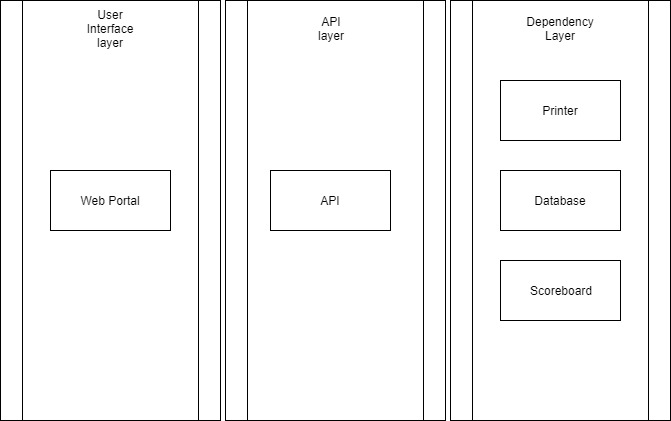
\includegraphics[width=\textwidth,height=\textheight,keepaspectratio]{dependencydiagram}
\subsection{Information viewpoint}
This sections contains information about our data structure and how the objects are connected.\\ \newline
\textbf{Entity Relationship Diagram} \\ \newline
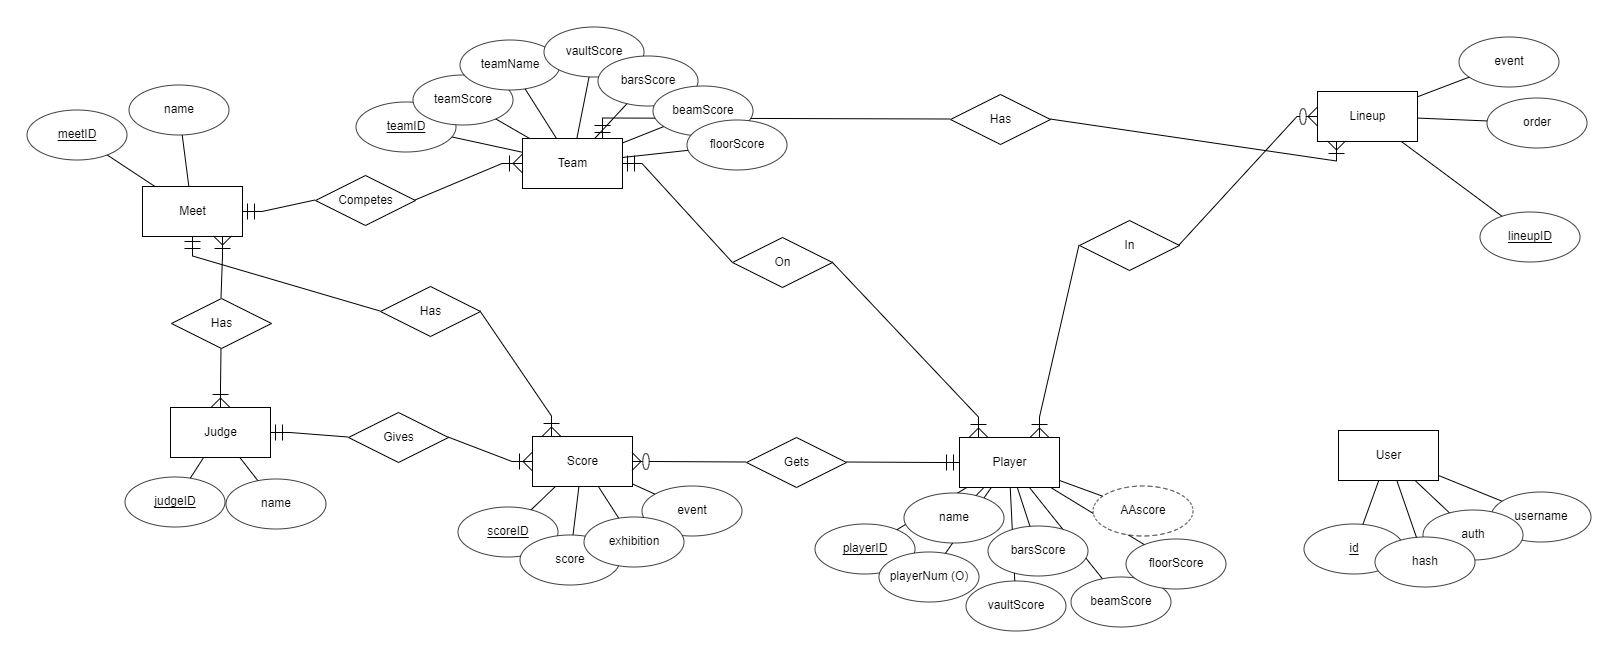
\includegraphics[width=\textwidth,height=\textheight,keepaspectratio]{gymnasticsDB.png}
\subsection{Patterns use viewpoint}
Due to the use of client-server, the common patterns that will be used are endpoints. These endpoints add a layer of abstraction that allows for developers to abstract common processes into easily callable functions.
\subsection{Interface viewpoint}
The interfaces that will be used will all be client side due to the server being an abstraction of processes. There will be three major interfaces, meet set-up, team set-up, and gymnast scoring. The meet set-up interface will allow for moderators to chose the number of teams and judges at the current meet. Next, the team set-up will allow for moderators to enter in data for each of the teams participating in the meets. Lastly the gymnast scoring interface will allow for either moderator or judge level accounts to send judges scores to the API.
\begin{figure}[H]
  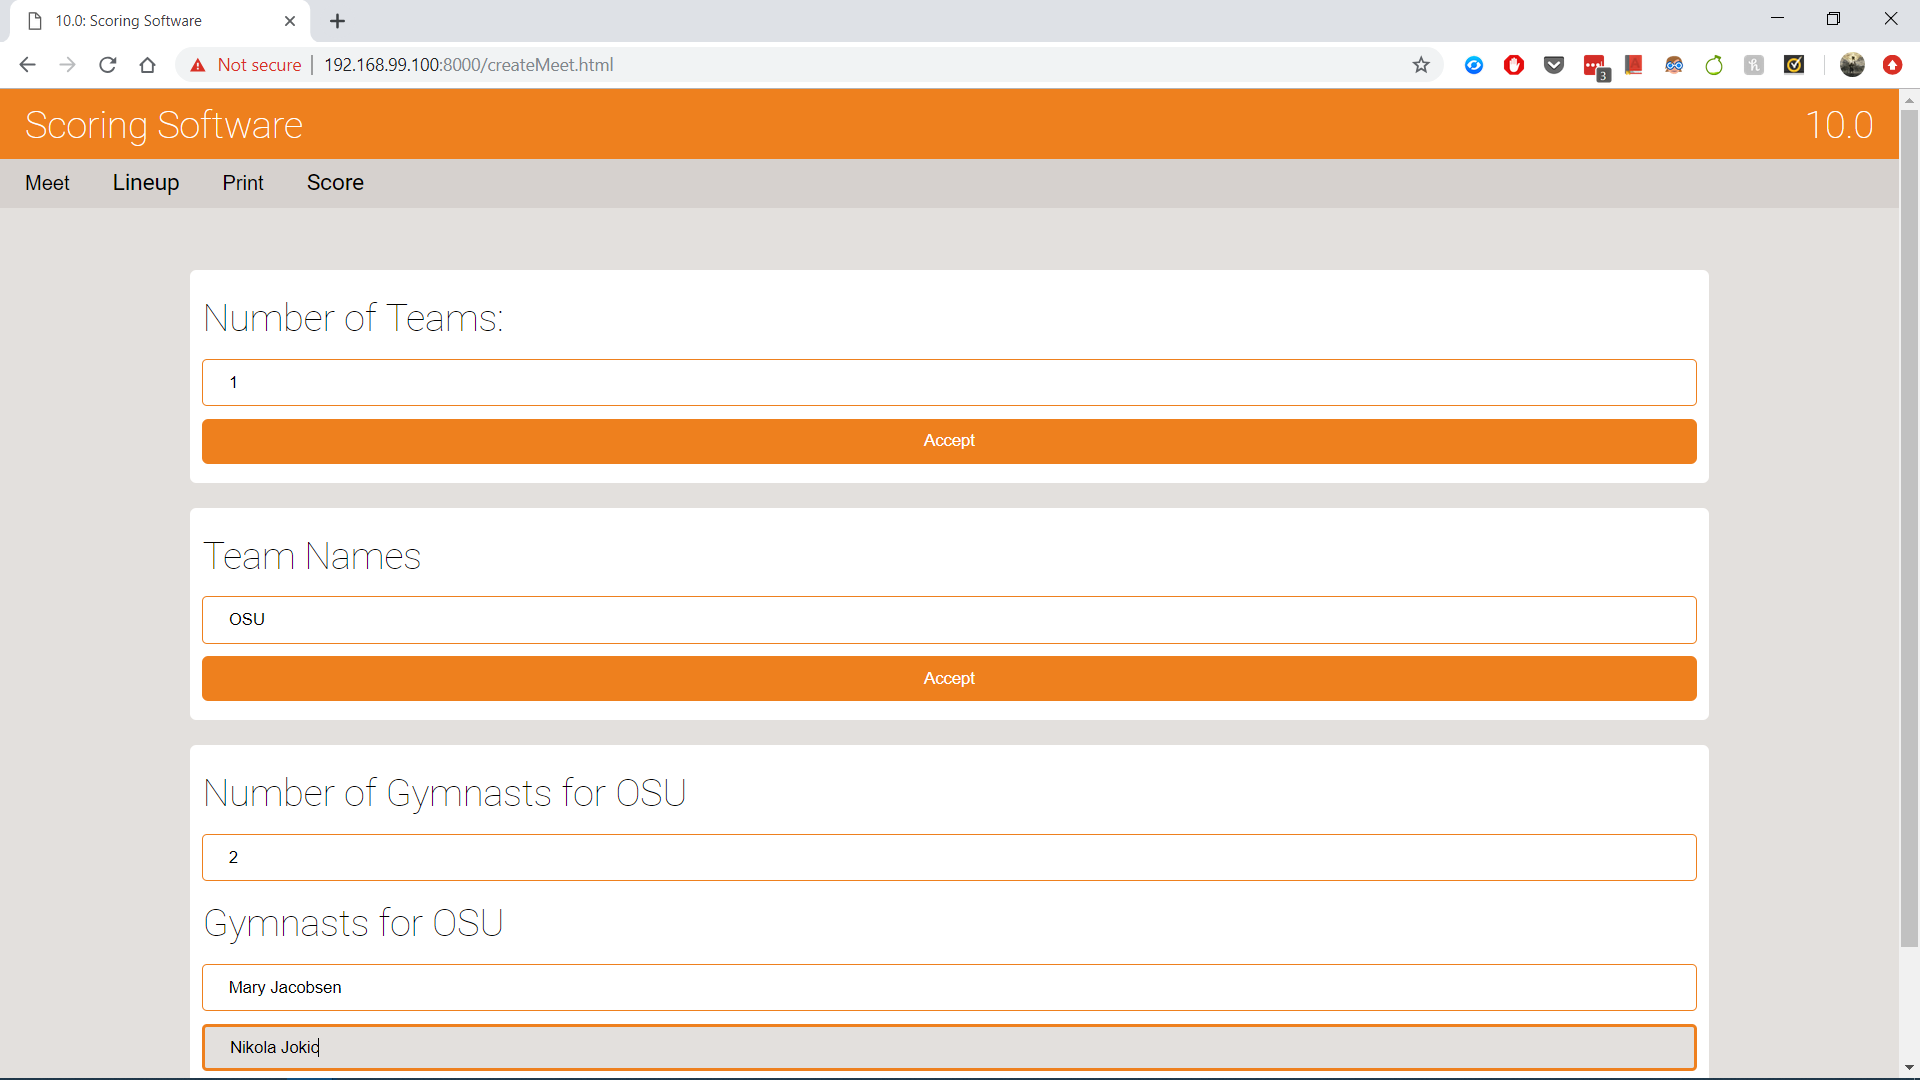
\includegraphics[width=\linewidth]{Capture.PNG}
  \caption{Create Meet Page}
  \label{fig:createMeet}
\end{figure}

\begin{figure}[H]
  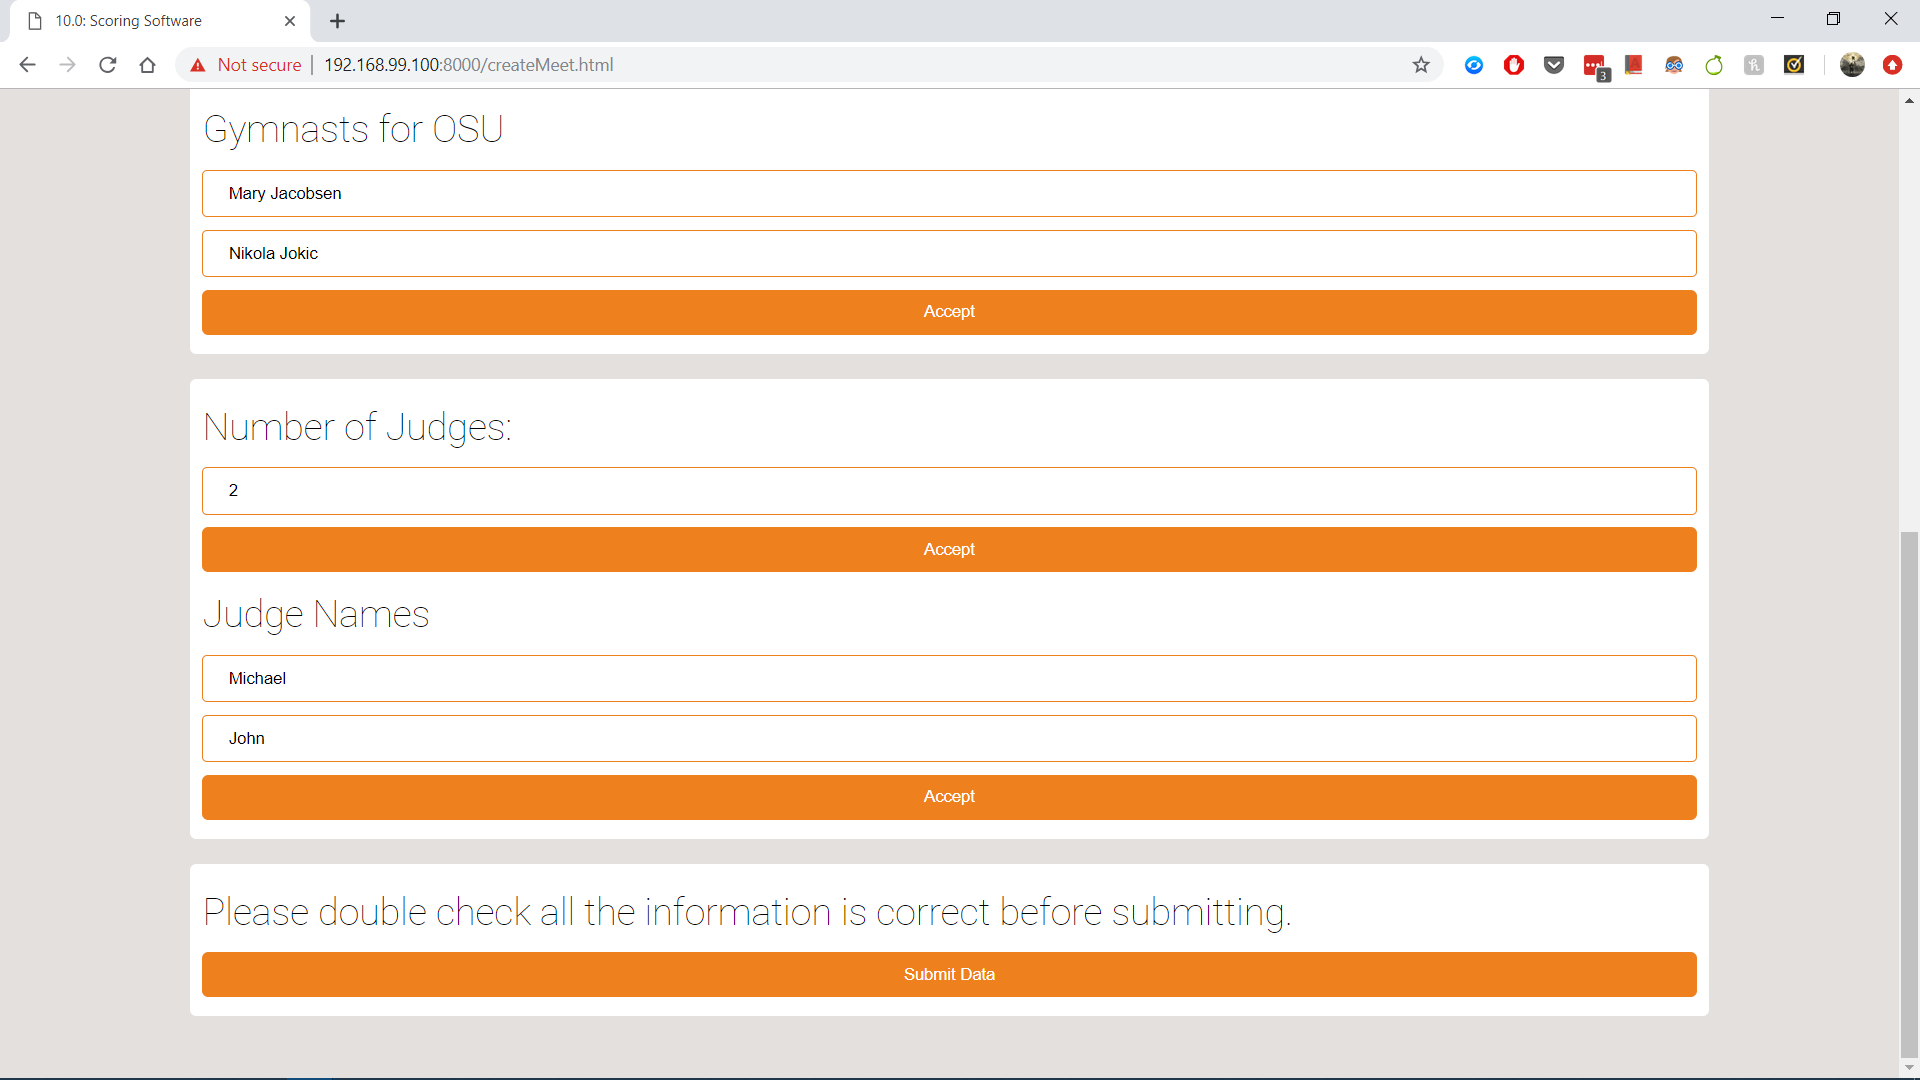
\includegraphics[width=\linewidth]{Capture2.PNG}
  \caption{Team set-up}
  \label{fig:teamsetup}
\end{figure}

\begin{figure}[H]
  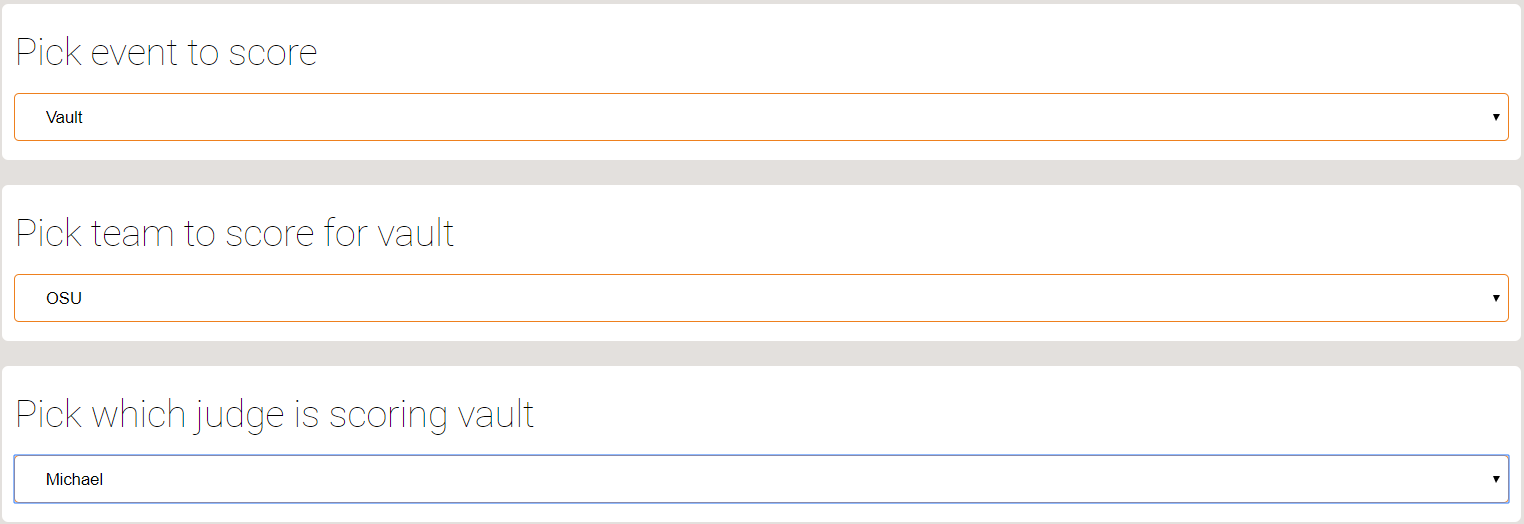
\includegraphics[width=\linewidth]{Capture5.png}
  \caption{Scoring interface}
  \label{fig:scoring}
\end{figure}

\subsection{Structure viewpoint}
The structure of this project can be exemplified by a client-server architecture. In essence, a client-server architecture is synchronized set of commands that are abstracted away from user to create ease of use for users while creating separation of key components to enhance portability and security. Our system will revolve around a central API that takes commands from a web portal that can be easily accessed.
\subsection{Interaction viewpoint}
Whenever the user want's to access data they must use the web portal to request information from the API. The API then acts as an intermediary to get and set data for the user and returns appropriate information. 
\subsection{State dynamics viewpoint}
Our program will have a multitude of modes that will be selected during the initial meet set-up. Once the meet has been set-up the it will be impossible to change the number of teams or the number of changes. The state will only be changeable during the beginning set-up phase.
\subsection{Algorithm viewpoint}
This viewpoint details the algorithms used in the design.
\begin{itemize}
    \item \textbf{Team Event Score}: The algorithm for getting team event scores works by iterating over the event lineup of that team. The top 5 scoring gymnasts have their scores added up and the total is returned.
    \item \textbf{All Around Score}: To ensure we don't qualify exhibitionists in the all around scoring, the all around score algorithm checks the exhibition flag before adding up scores for the all around event.
    \item \textbf{Average Player Score}: For each event there can be multiple judges. The scores from the judges are averaged and the result is the gymnast's final score.
\end{itemize}

\subsection{Resource viewpoint}
This section will contain every npm module we used and the purpose for why it was used. 
\subsubsection{NPM Modules}
\begin{itemize}
    \item Express
    \subitem a web framework for node with useful routing and middleware features
    \item Morgan
    \subitem HTTP request logger middleware for node.js
    \item Body-Parser
    \subitem Used to parse incoming request bodies
    \item Express-handlebars
    \subitem Used with express to create dynamic page content
    \item MySQL
    \subitem Used to make queries to the SQL database
    \item Client-sessions
    \subitem Used to keep track of session information such as current meet ID
    \item Cookie-parser
    \subitem Used to parse JSON data from client stored cookies
    \item JQuery
    \subitem Used for DOM Tree traversal and manipulation
    \item JS-cookie
    \subitem Used to handle client side cookies
    \item Handlebars (client-side)
    \subitem Client side handlebars module
\end{itemize}
\end{document}
